\documentclass{article}

\usepackage{geometry}
\usepackage{amsmath}
\usepackage{graphicx, eso-pic}
\usepackage{listings}
\usepackage{hyperref}
\usepackage{multicol}
\usepackage{fancyhdr}
\usepackage{tikz}
\pagestyle{fancy}
\fancyhf{}
\hypersetup{ colorlinks=true, linkcolor=black, filecolor=magenta, urlcolor=cyan}
\geometry{ a4paper, total={170mm,257mm}, top=40mm, right=20mm, bottom=20mm, left=20mm}
\setlength{\parindent}{0pt}
\setlength{\parskip}{0.5em}
\renewcommand{\headrulewidth}{0pt}
\AddToShipoutPictureBG{%
  \AtPageUpperLeft{%
    \raisebox{-\height}{\includegraphics[width=\paperwidth, height=30mm]{../headerarkav.png}}
  }
}
\rfoot{\thepage}
\lfoot{Competitive Programming - Arkavidia 8.0}
\lstset{
    basicstyle=\ttfamily\small,
    columns=fixed,
    extendedchars=true,
    breaklines=true,
    tabsize=2,
    prebreak=\raisebox{0ex}[0ex][0ex]{\ensuremath{\hookleftarrow}},
    frame=none,
    showtabs=false,
    showspaces=false,
    showstringspaces=false,
    prebreak={},
    keywordstyle=\color[rgb]{0.627,0.126,0.941},
    commentstyle=\color[rgb]{0.133,0.545,0.133},
    stringstyle=\color[rgb]{01,0,0},
    captionpos=t,
    escapeinside={(\%}{\%)}
}

\begin{document}

\begin{center}
    \section*{C. Crewmate dan Impostor} % ganti judul soal

    \begin{tabular}{ | c c | }
        \hline
        Batas Waktu  & 3s \\    % jangan lupa ganti time limit
        Batas Memori & 256MB \\  % jangan lupa ganti memory limit
        \hline
    \end{tabular}
\end{center}

\subsection*{Deskripsi}
Terdapat sebuah kelompok bermain yang beranggotakan $N$ orang yang dilabeli dengan nomor $1$ sampai $N$. Mereka akan bermain sebuah permainan bernama \textit{Amogus}.

Dalam permainan tersebut, tiap pemain akan mendapatkan salah satu dari dua buah peran, yaitu \textit{crewmate} dan \textit{impostor}. Dalam permainan tersebut, orang ke-$i$ menuduh orang ke-$A_i (A_i \neq i)$ sebagai seorang \textit{impostor}. Seorang \textit{impostor} pasti akan menuduh seorang \textit{crewmate}, sedangkan \textit{crewmate} bisa menuduh semua orang selain dirinya. Banyaknya \textit{crewmate} selalu lebih banyak dari pada banyaknya \textit{impostor}.

Arka merupakan seseorang di luar kelompok tersebut yang ingin menebak ada berapa banyak \textit{impostor} yang ada pada permainan tersebut. Karena keterbatasan informasi, Arka akan menebak nilai maksimal dari banyaknya \textit{impostor} yang mungkin. Anda diminta untuk membantu Arka menebak nilai tersebut.

\subsection*{Format Masukan}
Baris pertama terdiri dari sebuah bilangan $N$ ($2 \leq N \leq 10^5$), menyatakan banyaknya orang yang bermain.

Baris kedua terdiri dari $N$ buah bilangan $A_1, A_2, ..., A_n$ ($1 \leq A_i \leq N, A_i \neq i$), dengan orang ke-$A_i$ merupakan orang yang dituduh oleh orang ke-$i$ sebagai seorang \textit{impostor}. 

\subsection*{Format Keluaran}
Satu baris berisi nilai maksimal dari banyaknya \textit{impostor} yang mungkin.

\begin{multicols}{2}
\subsection*{Contoh Masukan 1}
\begin{lstlisting}
3
2 3 2
\end{lstlisting}
\columnbreak

\subsection*{Contoh Keluaran 1}
\begin{lstlisting}
1
\end{lstlisting}
\vfill
\null
\end{multicols}

\begin{multicols}{2}
\subsection*{Contoh Masukan 2}
\begin{lstlisting}
6
3 1 2 6 4 5
\end{lstlisting}
\columnbreak

\subsection*{Contoh Keluaran 2}
\begin{lstlisting}
2
\end{lstlisting}
\vfill
\null
\end{multicols}

\subsection*{Penjelasan}
Pada testcase pertama, salah satu konfigurasi yang mungkin ialah sebagai berikut.

\begin{center}
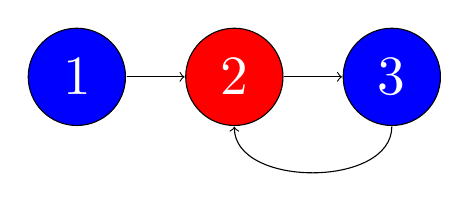
\begin{tikzpicture}
[impostor/.style = {draw, circle, fill=red, font=\color{white}, scale=2}, 
crewmate/.style = {draw,circle, fill=blue, font=\color{white}, scale=2}] 
\node[crewmate] (1) {$1$}; 
\node[impostor] (2) [right of =1]{$2$}; 
\node[crewmate] (3) [right of =2]{$3$};
\draw[->] (1)--(2);
\draw[->] (2)--(3);
\draw[->] (3) to [out=270, in=270](2);
\end{tikzpicture}
\end{center}
Gambar di atas menunjukkan bahwa orang pertama dan ketiga merupakan \textit{crewmate}, sedangkan orang kedua merupakan \textit{impostor}. Mudah dibuktikan bahwa tidak ada konfigurasi lain yang memiliki jumlah \textit{impostor} lebih banyak dari konfigurasi ini.\newline

Pada testcase kedua, salah satu konfigurasi yang mungkin ialah sebagai berikut.

\begin{center}
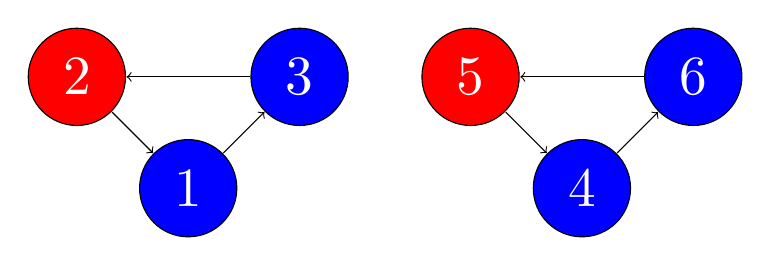
\begin{tikzpicture}
[impostor/.style = {draw, circle, fill=red, font=\color{white}, scale=2}, 
crewmate/.style = {draw,circle, fill=blue, font=\color{white}, scale=2}] 
\node[crewmate] (1) {$1$}; 
\node[impostor] (2) [above left of =1]{$2$}; 
\node[crewmate] (3) [above right of =1]{$3$};
\node[crewmate] (4) at (5,0) {$4$}; 
\node[impostor] (5) [above left of =4]{$5$}; 
\node[crewmate] (6) [above right of =4]{$6$};
\draw[->] (1)--(3);
\draw[->] (2)--(1);
\draw[->] (3)--(2);
\draw[->] (4)--(6);
\draw[->] (5)--(4);
\draw[->] (6)--(5);
\end{tikzpicture}
\end{center}
Gambar di atas menunjukkan bahwa orang kedua dan orang kelima merupakan \textit{impostor}. Mudah dibuktikan bahwa tidak ada konfigurasi lain yang memiliki jumlah \textit{impostor} lebih banyak dari konfigurasi ini.

\end{document}